\chapter{Multigrid} \label{chapter:multigrid_usage}
In this chapter we will introduce all the knowledge which is required for the usage of the multigrid. In order to understand the selection and cutting procedure which is the very heart of the multigrid class we refer to chapter \ref{chapter:multigrid_selection_and_cutting}.
\index{Multigrid}

\section{Overview}
A multigrid consists of a single basic grid region which defines the outer boundaries of the multigrid and multiple grid regions. Each of these grid regions can be equidistant, tangential or logarithmic. If the grid regions overlap with each other, they will be cut in such a way, that the grid resolution remains constant while crossing over the cutting point. It could also happen that a particular grid region is forced out by another grid region because the purpose of the former one is already served by the latter one. How this is done in detail will be part of chapter \ref{chapter:multigrid_selection_and_cutting}.

A multigrid is created in the following way (see listing \ref{lst:create_multigrid_sketch}). First it has to be initialized. Afterwards one can add, replace and remove multiple grid regions. This will be explained in detail in section \ref{sec:grid_regions}. Finally the member function \texttt{create} is invoked. Hereby the cutting and selection procedure will be performed and the multigrid will be created. 
\begin{lstlisting}[caption={Creating a multigrid},	label={lst:create_multigrid_sketch}]
multigrid mgrid;
... 
... //add, replace and remove grid regions
...
mgrid.create()
\end{lstlisting}
The multigrid is also derived from the grid class and can therefore be used exactly in the same way as the other grids (see section \ref{sec:using_the_grid_classes})

\section{Grid regions}\label{sec:grid_regions}
\index{Grid region}
In this chapter we will introduce the notion of a grid region. We will assume, that the purpose of a grid region is to resolve some feature of the integrand function which is located at a single point. This will be the center point of the grid region, $\omega_c$. Together with the left and right boundaries $\omega_l$ and $\omega_r$, the type of grid region (equidistant, tangential or logarithmic) and the grid region parameters (e.g. $\omega_k$ and $\omega_0$ for the loggrid) these are the defining properties of a grid region. The grid region is implemented as a class named \texttt{gridRegion} and is defined in the file \texttt{multigrid.h}. Its defining member variables are shown in table \ref{tab:grid_region_defining_members}.
\begin{table}[h]
	\begin{center}
		\begin{tabular}{ll}
		Name & Description \\ 
		\hline
		$\omega_c$  & Center point \\
		$\omega_l$  & Lower boundary \\
		$\omega_r$  & Upper boundary \\
		\texttt{type}  & Type of grid region \\
		\texttt{id}  & Name of the grid region (optional) \\
		 $\dots$ & Grid region parameters (e.g. $\omega_k$ and $\omega_0$ for the loggrid) \\
		\end{tabular}
	\end{center}
	\caption{Defining properties of the grid region}
	\label{tab:grid_region_defining_members}
\end{table}

It is obvious, that a possible cutting point can not be arbitrarily narrow to the center point $\omega_c$. For example in the loggrid case, for numerical reasons at least three points of the exponential grid regions must survive in order to have a starting, an intermediate and an endpoint of this region. Also the corresponding weights should not be smaller than the machine precision. Therefore one introduces a buffer region around $\omega_c$ which is defined by its upper and lower boundaries $\omega_+$ and $\omega_-$. In section \ref{sec:cutting_procedure} we will see, that in order to calculate the cutting point according to the grid point density (grid resolution) the maximal grid resolution on both sides of the center point, $d\omega_l$ and $d\omega_r$, is necessary. Hereby we assume that the grid point density is monotonically increasing from the boundaries towards the center of the grid region. (This is true for all three kinds of grids from chapter \ref{chapter:simple_grids}). Table \ref{tab:grid_region_derived_members} shows the relevant derived properties of the grid region class, i.e. they are calculated directly out of the defining properties.
\begin{table}[h]
	\begin{center}
		\begin{tabular}{ll}
		Name & Description \\ 
		\hline
		$\omega_+$  & Upper boundary of the buffer region around $\omega_c$ \\
		$\omega_-$  & Lower boundary of the buffer region around $\omega_c$ \\
		$d\omega_l$  & Maximal resolution left to $\omega_c$ \\
		$d\omega_r$  & Maximal resolution right to $\omega_c$ \\
		\end{tabular}
	\end{center}
	\caption{Relevant derived properties of the grid region}
	\label{tab:grid_region_derived_members}
\end{table}

Note that there are actually more member variables. But since they will never appear to the user we will not discuss them here. In the following we will introduce the different kinds of grid regions. There are equidistant, tangential and logarithmic grid regions. Naturally, the boundaries of a particular grid region $\omega_l$ and $\omega_r$ will correspond to the boundary $\omega_{min}$ and $\omega_{max}$ of the simple grids from chapter \ref{chapter:simple_grids}. In table \ref{tab:grid_region_types} the mapping from the grid class member variables to the grid region member variables is shown. As mentioned earlier, the boundaries of the buffer region around the center point are chosen such, that there will be 3 points left. In the case of the logarithmic grid region, the buffer region always includes the linear region II of the loggrid. Note, that the center point of the equidistant grid region can be chosen arbitrarily.
\begin{table}[h]
	\begin{center}
		\begin{tabular}{llll}
		Grid region & equidistant & tangential & logarithmic  \\ 
		variable    &             &            &              \\
		\hline 
		$\omega_c$    & -               & $\omega_c$     & $\omega_k$     \\
		$\omega_l$    & $\omega_{min}$  & $\omega_{min}$ & $\omega_{min}$ \\
		$\omega_r$    & $\omega_{max}$  & $\omega_{max}$ & $\omega_{max}$ \\
		\texttt{type} & \texttt{'equi'} & \texttt{'tan'} & \texttt{'log'} \\
		$\omega_+$         & $\omega_c+3d\omega$ & $\omega_c+3c\Delta u$ & $\omega(i=N_l+N_k+3)$ \\
		$\omega_-$         & $\omega_c-3d\omega$ & $\omega_c-3c\Delta u$ & $\omega(i=N_l-3)$  \\
		$d\omega_l$  & $d\omega$ & $c\Delta u$ & see Appendix \ref{sec:app_loggrid_max_resolution} \\
		$d\omega_r$  & $d\omega$ & $c\Delta u$ & see Appendix \ref{sec:app_loggrid_max_resolution} \\
		\end{tabular}
	\end{center}
	\caption{Relation of grid class and grid region member variables}
	\label{tab:grid_region_types}
\end{table}

\subsection{Adding grid regions}\label{subsec:grid_region_adding}
\index{Grid region!equidistant}
\index{Grid region!tangential}
\index{Grid region!logarithmic}
\index{Grid region!add}
In this section we introduce the syntax for adding grid regions to the multigrid. (See section \ref{subsec:grid_region_examples} for examples).
An equidistant grid region consists of an instance of an equigrid (see \ref{sec:equigrid}). It is added to the multigrid by the member function 
\begin{lstlisting}
void add_gr_equi
\end{lstlisting}
Its arguments are shown in table \ref{tab:add_gr_equi}.

\begin{table}[h]
	\begin{center}
		\begin{tabular}{lll}		
		Argument  & Type & Description \\ \hline
		\nth{1}   & \texttt{int}    & Number of grid points ($M$) \\ 
		\nth{2}   & \texttt{double} & Lower boundary ($\omega_l$) \\ 
		\nth{3}   & \texttt{double} & Upper boundary ($\omega_r$) \\ 
		\nth{4}   & \texttt{double} & Center point ($\omega_c$) \\ 
		(\nth{5}) & \texttt{string} & Name of the grid region (\texttt{id})(optional)\\ 
		\end{tabular}
	\end{center}
	\caption{Arguments of the member function \texttt{add\_gr\_equi}}
	\label{tab:add_gr_equi}
\end{table}

A tangential grid region consists of an instance of a tangrid (see \ref{sec:tangrid}). It is added to the multigrid by the member function 
\begin{lstlisting}
void add_gr_tan
\end{lstlisting}
Its arguments are shown in table \ref{tab:add_gr_tan}.

\begin{table}[h]
	\begin{center}
		\begin{tabular}{lll}		
		Argument  & Type & Description \\ \hline
		\nth{1}   & \texttt{int}    & Number of grid points ($M$) \\ 
		\nth{2}   & \texttt{double} & Lower boundary ($\omega_l$) \\ 
		\nth{3}   & \texttt{double} & Upper boundary ($\omega_r$) \\ 
		\nth{4}   & \texttt{double} & Center point ($\omega_c$) \\ 
		\nth{5}   & \texttt{double} & Controls sharpness ($c$) \\ 
		(\nth{6}) & \texttt{string} & Name of the grid region (\texttt{id})(optional)\\ 
		\end{tabular}
	\end{center}
	\caption{Arguments of the member function \texttt{add\_gr\_tan}}
	\label{tab:add_gr_tan}
\end{table}

A logarithmic grid region consists of an instance of a loggrid (see \ref{sec:loggrid}). It is added to the multigrid by the member function 
\begin{lstlisting}
void add_gr_log
\end{lstlisting}
Its arguments are shown in table \ref{tab:add_gr_log}.

\begin{table}[h]
	\begin{center}
		\begin{tabular}{lll}		
		Argument  & Type & Description \\ \hline
		\nth{1}   & \texttt{int}    & Number of grid points in region I ($N_l$) \\ 
		\nth{2}   & \texttt{int}    & Number of grid points in region III ($N_r$) \\ 
		\nth{3}   & \texttt{double} & Lower boundary ($\omega_l$) \\ 
		\nth{4}   & \texttt{double} & Upper boundary ($\omega_r$) \\ 
		\nth{5}   & \texttt{double} & Center point ($\omega_k$) \\ 
		\nth{6}   & \texttt{double} & Half width of region II ($\omega_0$) \\ 
		(\nth{7}) & \texttt{string} & Name of the grid region (\texttt{id})(optional)\\ 
		\end{tabular}
	\end{center}
	\caption{Arguments of the member function \texttt{add\_gr\_log}}
	\label{tab:add_gr_log}
\end{table}

\subsection{Replacing and removing grid regions}\label{subsec:grid_region_replace_remove}
\index{Grid region!equidistant}
\index{Grid region!tangential}
\index{Grid region!logarithmic}
\index{Grid region!replace}
\index{Grid region!remove}
After adding a lot of grid regions to the multigrid there may be a situation were one wants to change only a single grid region out of many. This can be achieved by replacing that particular grid region by another one with different parameters.
We have seen, that if a grid region is added to the multigrid, it is optional to give a name to this grid region. In contrast to that, you can only replace or remove grid regions which have a name. One can check if a grid region with the name \texttt{id} exists, by calling the member function
\begin{lstlisting}
bool gr_exists(string id)
\end{lstlisting}
If this is the case one can remove it by
\begin{lstlisting}
void rem_gr(string id)
\end{lstlisting}
In order to replace a grid region by one with the same name but different attributes one calls one of the replace member functions
\begin{lstlisting}
void replace_gr_equi(...)
void replace_gr_tan(...)
void replace_gr_log(...)
\end{lstlisting}
where the arguments are exactly the same as for the add functions (see tables \ref{tab:add_gr_equi}, \ref{tab:add_gr_tan} and \ref{tab:add_gr_log}). The only difference is, that for the replace functions you definitely have to give the name of the grid region which is to be replaced, as the \texttt{id} argument.

\subsection{Examples}\label{subsec:grid_region_examples}
\index{Grid region!add}
\index{Grid region!remove}
\index{Grid region!replace}

In this section we will show in some examples how the different types of grid regions can be added, replaced or removed from the multigrid. 

\begin{lstlisting}[caption={Example for adding grid regions},label={lst:add_gr}]
multigrid mgrid;
mgrid.add_gr_equi(100, -1, 1, 0);
mgrid.add_gr_tan(100, 0.2, 0.5, 0.3, 0.01);
mgrid.add_gr_log(100, 100, 0.4, 0.7, 0.6, 1E-6, "gr");
mgrid.create();
\end{lstlisting}

In listing \ref{lst:add_gr} we show an example for the adding of grid regions. At first, an equidistant grid region with $100$ points from $-4$ to $4$ is added to the multigrid. This defines the basic grid region and therefore the boundaries of the multigrid. The center point of a basic grid region (here at $0$) is obsolete because there is no cutting for the basic grid region. Afterwards a tangential grid region with $100$ points from $0.2$ to $0.5$ with a center point at $0.3$ is added. The parameter $c$ is $0.01$ here. Finally a third, logarithmic grid region is added. It overlaps with the tangential grid region and an appropriate cutting point will be calculated such that the grid resolution remains constant across the cutting point. The logarithmic grid region is named   ``gr'' and has 100 points in both of the exponential grid regions. Its boundaries are at $0.4$ and $0.7$, its center point $\omega_k$ is at $0.6$ and the half width of the linear region $\omega_0$ is $10^{-6}$. The resulting multigrid is shown in figure \ref{fig:example_add_gr}.
\begin{figure}[h]
	\centering
	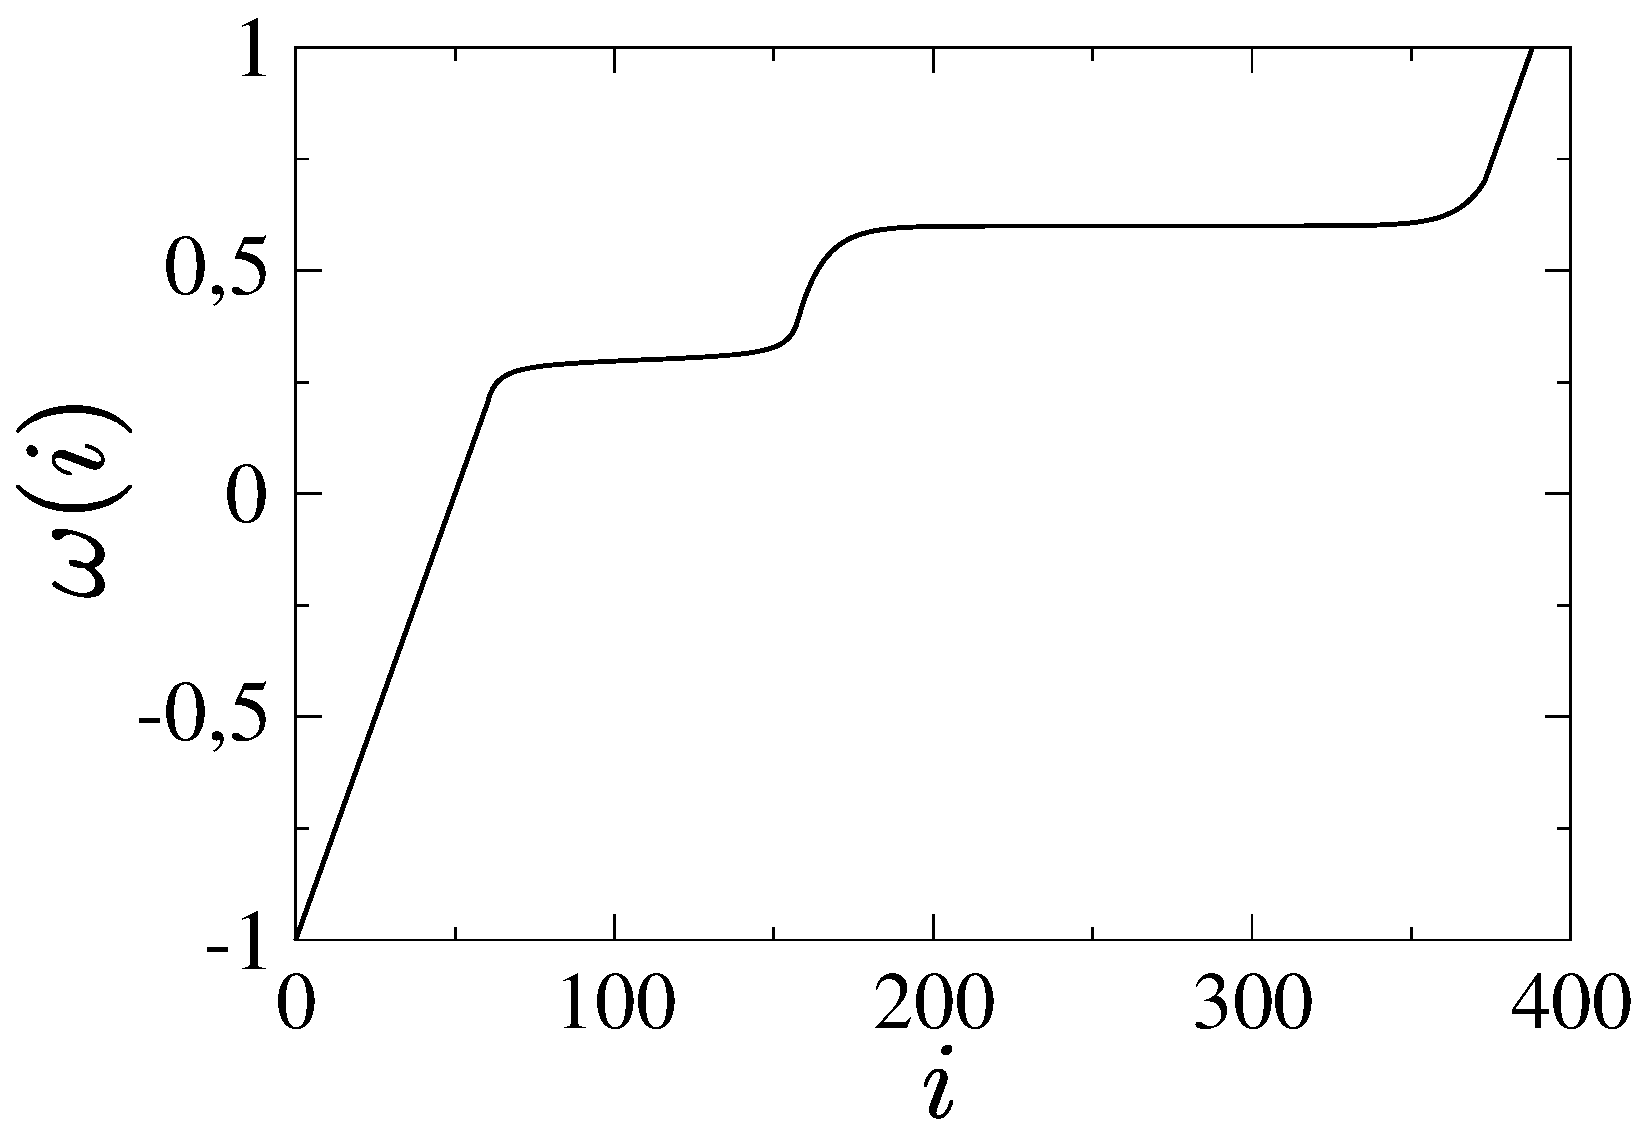
\includegraphics[width=0.5\textwidth]{pics/example_add_gr.eps}
	\caption{Multigrid corresponding to listing \ref{lst:add_gr}}
	\label{fig:example_add_gr}
\end{figure}

\begin{lstlisting}[caption={Example for replacing a grid region},label={lst:replace_gr}]
mgrid.replace_gr_equi(100, -0.5, 0.0, "gr");
mgrid.create();
\end{lstlisting}

In listing \ref{lst:replace_gr} the logarithmic grid region named ``gr'' from the multigrid instance ``mgrid'' is replace by an equidistant grid region with the same name. In order to apply this change the create function has to be invoked once again. Note, that if one tries to replace a non-existing grid region, this will result in a simple adding of the desired grid region. The resulting multigrid is shown in figure \ref{fig:example_replace_gr}.
\begin{figure}[h]
	\centering
	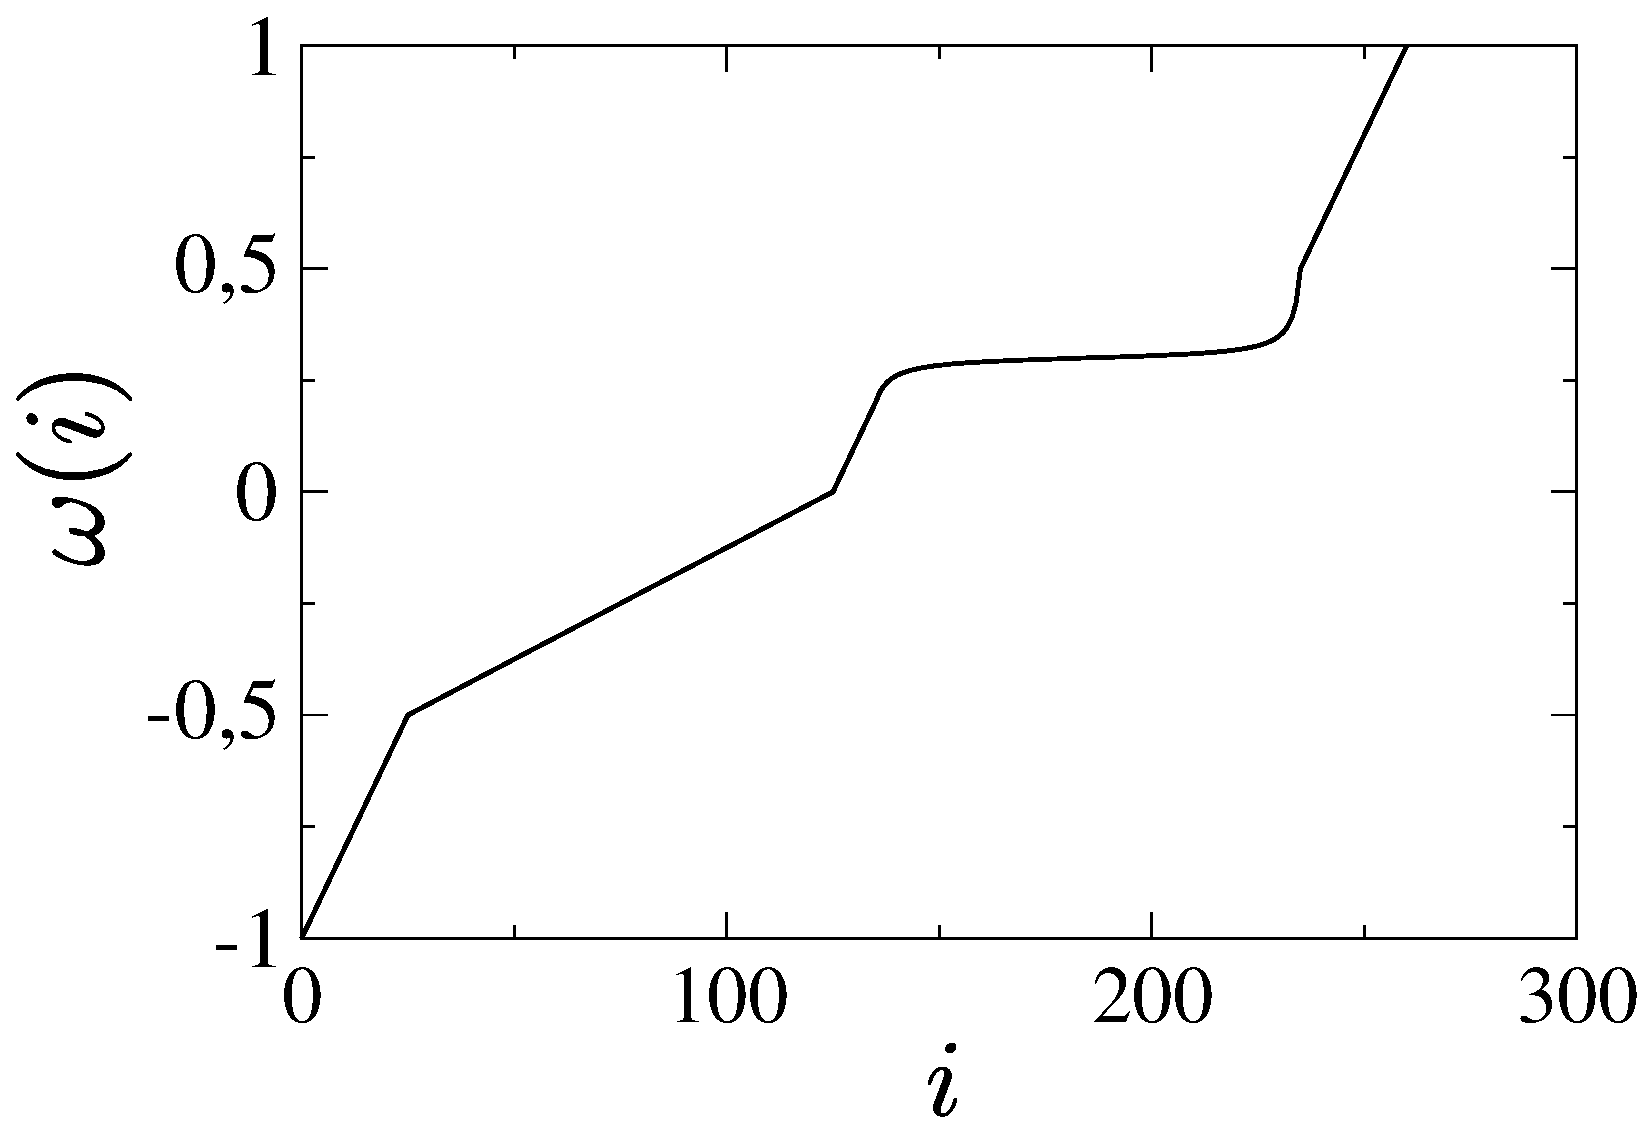
\includegraphics[width=0.5\textwidth]{pics/example_replace_gr.eps}
	\caption{Multigrid corresponding to listing \ref{lst:replace_gr}}
	\label{fig:example_replace_gr}
\end{figure}

\subsection{More convenient ways of adding and replacing}\label{subsec:wrapper}
There are more convenient ways of adding or replacing equidistant and logarithmic grid regions. For the former it might be desirable to specify the grid resolution $d\omega$ instead of the number of grid points $M$. And for the latter it would be convenient just to give the maximal resolution at the center point $d\omega_{min}$ and the minimal resolution at the boundaries $d\omega_{max}$ together with the center point $\omega_k$ and the half width of the grid region $\omega_1=(\omega_r-\omega_l)/2$ instead of specifying the grid point numbers $N_l$ and $N_r$, $\omega_0$ and the boundaries $\omega_l$ and $\omega_r$. Note that hereby we made the logarithmic grid region symmetric around the center point. There are wrapper functions for adding and replacing equidistant and logarithmic grid regions which possess these properties. They are shown in the tables \ref{tab:add_gr_equi_wrapper} and \ref{tab:add_gr_log_wrapper}. For examples see chapter \ref{chapter:quick_start_guide}, where these wrapper functions are used throughout the entire chapter. Note that the center point of the equidistant grid region is naturally chosen to be $\omega_c=(\omega_r-\omega_l)/2$.

\begin{table}[h]
	\begin{center}
		\begin{tabular}{lll}		
		Argument  & Type & Description \\ \hline
		\nth{1}   & \texttt{double} & Lower boundary ($\omega_l$) \\ 
		\nth{2}   & \texttt{double} & Upper boundary ($\omega_r$) \\ 
		\nth{3}   & \texttt{double} & Resolution ($d\omega$) \\
		(\nth{4}) & \texttt{string} & Name of the grid region (\texttt{id})(optional)\\ 
		\end{tabular}
	\end{center}
	\caption{Arguments of the wrapper functions \texttt{add\_gr\_equi} and \texttt{replace\_gr\_equi}}
	\label{tab:add_gr_equi_wrapper}
\end{table}

\begin{table}[h]
	\begin{center}
		\begin{tabular}{lll}		
		Argument  & Type & Description \\ \hline
		\nth{1}   & \texttt{double} & Center point ($\omega_k$) \\ 
		\nth{2}   & \texttt{double} & Half width ($\omega_1$) \\ 
		\nth{3}   & \texttt{double} & Maximal resolution at the center point ($d\omega_{min}$)\\ 
		\nth{4}   & \texttt{double} & Minimal resolution at the boundaries ($d\omega_{max}$)\\ 
		(\nth{5}) & \texttt{string} & Name of the grid region (\texttt{id})(optional)\\ 
		\end{tabular}
	\end{center}
	\caption{Arguments of the wrapper functions \texttt{add\_gr\_log} and \texttt{replace\_gr\_log}}
	\label{tab:add_gr_log_wrapper}
\end{table}

For the logarithmic grid region the mapping from maximal and minimal resolutions $d\omega_{max}$ and $d\omega_{min}$ to the loggrid variables $\omega_0$, $N_l$ and $N_r$ is determined by the following equations:
\begin{align*}
	\omega_0 & = \frac{\omega_1 d\omega_{min}}{d\omega_{max}}\\
        N_l=N_r& =log\left(\frac{\omega_1}{\omega_0}\right) \frac{\omega_1}{d\omega_{max}}
\end{align*}

\section{Fundamental and special grid regions}\label{sec:fundamental_and_special_grid_regions}
\index{Fundamental grid regions}
\index{Special grid regions}
As it was explained in the beginning of this chapter, the base grid region defines the outer boundaries of the multigrid. A grid region which is added to the multigrid after the base grid region is called fundamental grid region (FGR). The selection and cutting procedure will remove all overlaps between the FGR (see chapter \ref{chapter:multigrid_selection_and_cutting}). By adding such an FGR, all the grid points of the base grid which lie inside the boundaries of the FGR will be removed and replaced by the grid points of the FGR.

Up to now, the base grid has to be one of the grid regions based on the simple grids: equidistant, tangential or logarithmic. But in principle there is nothing to be said against using a multigrid itself as a base grid. This is achieved by letting the basic grid region and the FGR go through the selection and cutting procedure and building a ``multigrid''-like grid which is called the fundamental grid. The fundamental grid serves as a ``base'' grid for additional grid regions which will be called special grid regions (SGR). These special grid regions are added, replaced or removed exactly in the same way as for the FGR. The only difference is, that one has to replace the '\texttt{gr}' in the member functions of section \ref{sec:grid_regions} by a '\texttt{sgr}'.
\begin{lstlisting}[caption={Example for adding special grid regions},label={lst:add_sgr}]
	multigrid mgrid;
	mgrid.add_gr_equi(100, -1, 1, 0);
	mgrid.add_gr_tan(100, 0.2, 0.5, 0.3, 0.01);
	mgrid.add_gr_log(100, 100, 0.4, 0.7, 0.6, 1E-6, "gr");
	mgrid.add_sgr_equi(0.5, 0.8, 0.001);
	mgrid.create();
\end{lstlisting}
Listing \ref{lst:add_sgr} is exactly the same as listing \ref{lst:add_gr} but with an additional adding of a special equidistant grid region from $0.5$ to $0.8$ with resolution $0.001$. (Note, that we used one of the wrapper functions from section \ref{subsec:wrapper} here.) This SGR will just ``bump away'' most parts of the logarithmic grid region, even though its maximal resolution ($10^{-6})$ is much higher than the one of the SGR ($10^{-4}$). Therefore one can use SGR for ``tricking'' the selection and cutting procedure to some extent. It is needless to say, that if you add multiple SGR they will also run through a selection and cutting procedure. The resulting multigrid of listing \ref{lst:add_sgr} is shown in figure \ref{fig:example_add_sgr}.
\begin{figure}[h]
	\centering
	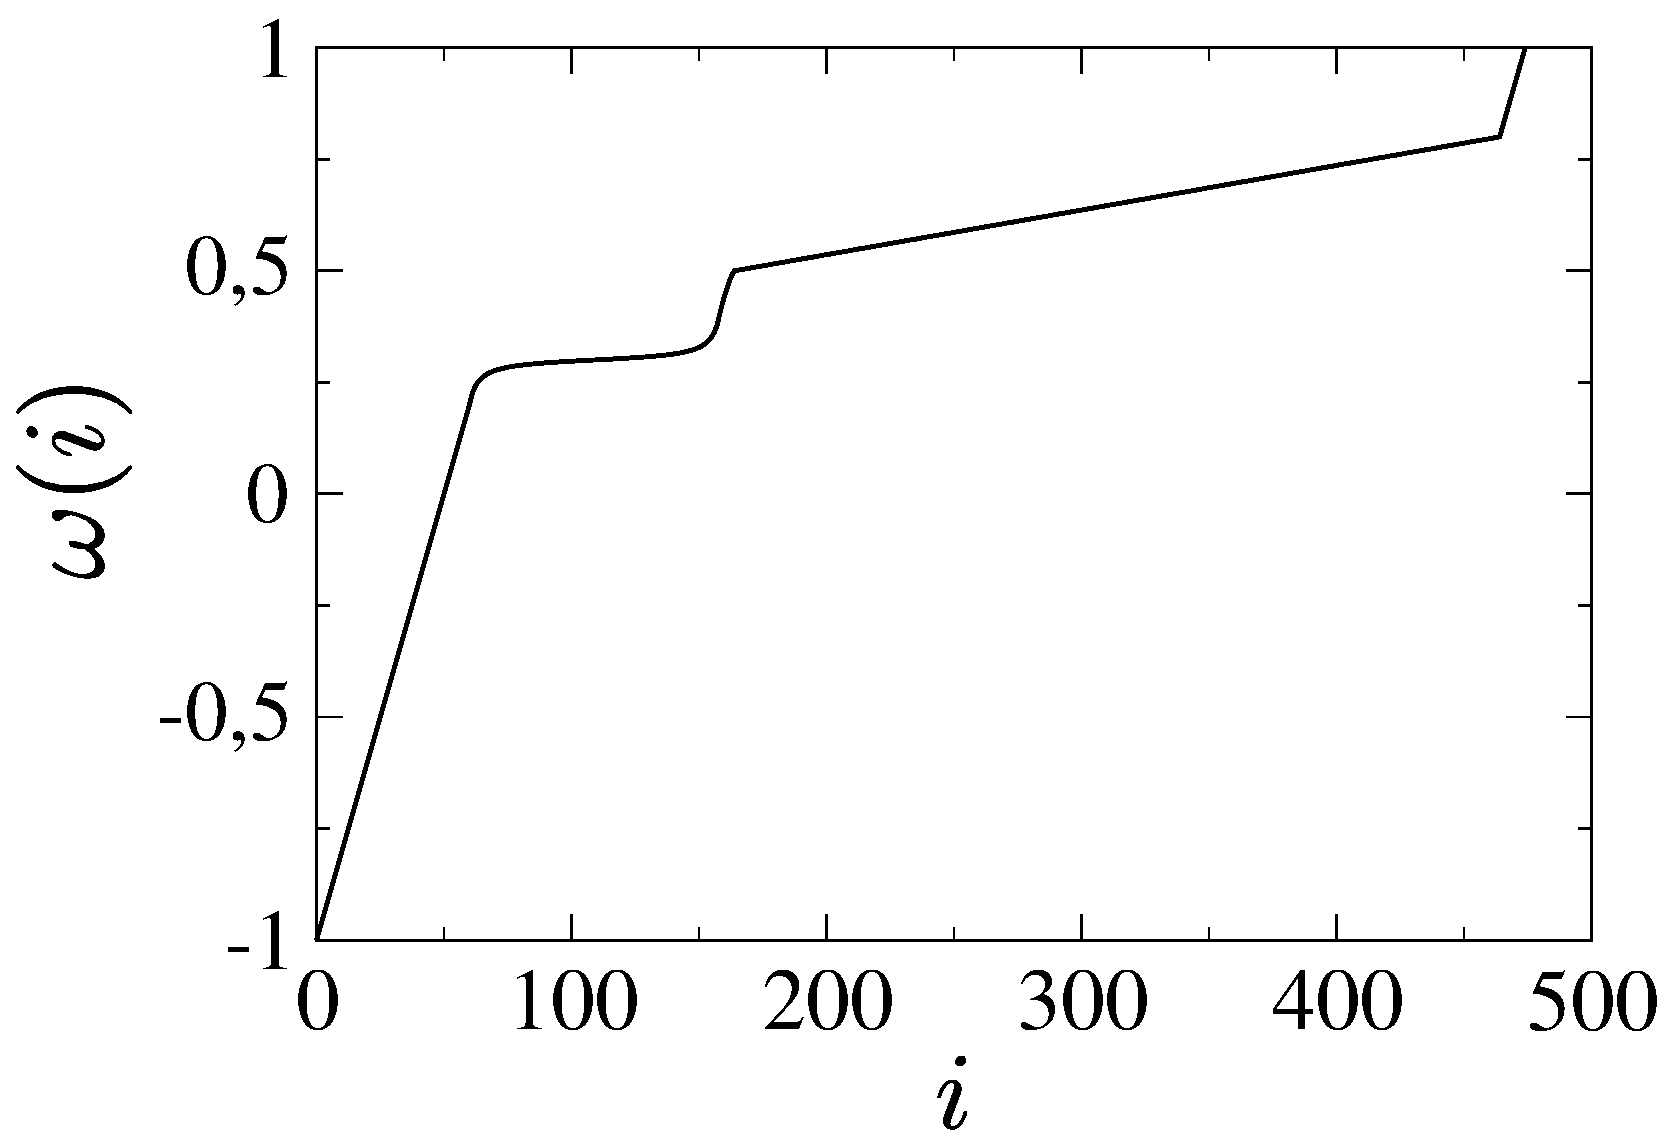
\includegraphics[width=0.5\textwidth]{pics/example_add_sgr.eps}
	\caption{Multigrid corresponding to listing \ref{lst:add_sgr}}
	\label{fig:example_add_sgr}
\end{figure}

